\def\CTeXPreproc{Created by ctex v0.2.9, don't edit!}
%\documentclass{beamer}
\documentclass[%handout,
xcolor=pdftex]{beamer}
\mode<presentation> {
  \usetheme{Warsaw}
  \setbeamercovered{transparent}
}
\let\Tiny=\tiny
\usetheme{Singapore}
\usecolortheme{dolphin}
\usepackage{amsmath}
\usepackage{textcomp}
\usepackage{amssymb}
\usepackage{amsthm}
\usepackage{graphicx}
\usepackage{color}
\usepackage{lipsum}
\usepackage{hyperref}
\usepackage{multirow}
\usepackage{bm}
\DeclareMathSymbol{\Phi}{\mathalpha}{operators}{8}
%\setbeamertemplate{headline}{}
\setbeamertemplate{footline}[page number]
\newcommand\Fontvi{\fontsize{9pt}{8}\selectfont}
\newcommand\Fontvii{\fontsize{7pt}{8}\selectfont}
\newcommand{\backupbegin}{
   \newcounter{finalframe}
   \setcounter{finalframe}{\value{framenumber}}
}
\newcommand{\backupend}{
   \setcounter{framenumber}{\value{finalframe}}
}\newtheorem{proposition}{Proposition}
\title{Unit 20: Discrete Fourier Transform and Periodogram}
\author[STAT 5170: Applied Time Series, Unit 20]{Jeffrey Woo}
\institute{Department of Statistics, University of Virginia}
\date{Spring 2020}  %USE ADITYA LECTURE 23

\AtBeginSubsection[] {
  \begin{frame}<beamer>{Outline}
    \tableofcontents[currentsection,currentsubsection]
  \end{frame}
}



\begin{document}


\frame{\titlepage}


\begin{frame}
\frametitle{Readings for Unit 20}

Textbook chapter 4.3.

\end{frame}



\begin{frame}
\frametitle{Last Unit}
\begin{enumerate}
\item Autocovariance generating function for ARMA processes.
\item Rational spectrum representation for ARMA processes.
\end{enumerate}
\end{frame}

\begin{frame}
\frametitle{This Unit}
\begin{enumerate}
\item Discrete Fourier Transform
\item Periodogram
\end{enumerate}
\end{frame}

\begin{frame}
\frametitle{Motivation}

So far, we've looked at the spectral density, which is a population quantity. We'll next consider the sample version: the periodogram.

\end{frame}

\section{Discrete Fourier Transform}
\frame{\tableofcontents[currentsection]}

\begin{frame}
\frametitle{Discrete Fourier Transform}

Given data $x_1,x_2,\ldots,x_n$, we define
the discrete Fourier transform (DFT) as

\begin{equation} \label{eq:DFT}
d(\omega_j)=n^{-1/2} \sum_{t=1}^n x_t e^{-2 \pi i \omega_j t}
\end{equation}

where $\omega_j= j/n, j=0,1,\ldots,n-1$, and the frequencies $\omega_j = j/n$ are called the Fourier or \underline{\hspace{40 mm}}.
\end{frame}

\begin{frame}
\frametitle{Discrete Fourier Transform}

The difference between the DFT (\ref{eq:DFT}) and the Fourier transform
in Unit 18 is that the DFT does the computation for
discrete frequency $\omega_j$ while the Fourier transform does for
all frequencies $-1/2 \leq \omega_j \leq 1/2$.

\end{frame}

\begin{frame}
\frametitle{Discrete Fourier Transform}

Using Euler's formula $e^{i\alpha}=cos(\alpha)+i sin(\alpha)$, we could also write the DFT (\ref{eq:DFT}) as

\begin{equation} \label{eq:DFT2}
d(\omega_j)=n^{-1/2} \sum_{t=1}^n x_t cos(2 \pi \omega_j t)-i n^{-1/2} \sum_{t=1}^n x_t sin(2 \pi \omega_j t).
\end{equation}

\end{frame}

\begin{frame}
\frametitle{Discrete Fourier Transform}

The real part of (\ref{eq:DFT2}) is identified as the cosine transform $d_c(\omega_j)$ and the imaginary part as the sine transform $d_s(\omega_j)$.  We could write the DFT (\ref{eq:DFT}) as
$$
d(\omega_j)=d_c(\omega_j)-i d_s(\omega_j).
$$
\end{frame}

\section{Periodogram}
\frame{\tableofcontents[currentsection]}

\begin{frame}
\frametitle{Periodogram}

The periodogram is defined to be

\begin{equation} \label{eq:period}
I(\omega_j) =|d(\omega_j)|^2.
\end{equation}

i.e. the squared modulus of the DFT (\ref{eq:DFT}). Recall that $|a+ib|^2=a^2+b^2$.  Therefore,
$$
I(\omega_j)=\left(d_c(\omega_j)\right)^2+\left(-d_s(\omega_j)\right)^2=d^2_c(\omega_j)+d^2_s(\omega_j)
$$

\end{frame}


\begin{frame}
\frametitle{A Few Notes about Complex Numbers}

\begin{eqnarray*}
\overline{a+ib}&=&a-ib \quad (\mbox{complex conjugate},~~ \overline{a}=a\mbox{~for real number~}a.) \\
|a+ib|^2&=&a^2+b^2=(a+ib)\overline{(a+ib)}. \quad (|z| \mbox{~is the modulus of~} z.) \\
\overline{z_1 z_2} &=& \overline{z_1}\text{  } \overline{z_2}, \quad
\mbox{for two complex numbers~} z_1,z_2.
\end{eqnarray*}

\end{frame}

\begin{frame}
\frametitle{Periodogram as Sample Version of Spectral Density}



\end{frame}

\begin{frame}
\frametitle{Inverse Fourier Transform}

Another useful property is the inverse Fourier transform
\begin{eqnarray*}
x_t&=&n^{-1/2} \sum_{j=0}^{n-1} d(\omega_j) e^{2 \pi i \omega_j t} \\
&=& \\
&=& \\
&=& \\
&=&
\end{eqnarray*}
where $a_0=\bar{x}=(x_1+\cdots+x_n)/n$, and we have assumed for
simplicity that $n$ is odd and $m=(n-1)/2$.

\end{frame}

\begin{frame}
\frametitle{Interpreting the Periodogram}

We can think of the inverse Fourier transform as a
regression of $x_t$ on  sines and cosines with the coefficients
equal to $2/\sqrt{n}$ times the sine part and the cosine part
of the Fourier transforms respectively. Therefore,
$d_c(\omega_j)$ and $d_s(\omega_j)$ measure the contribution the frequency $\omega_j$ has in \underline{\hspace{45 mm}} in
the time series. The bigger $d_c(\omega_j)$ and
$d_s(\omega_j)$, the greater the contribution from the
frequency $\omega_j$.

\end{frame}

\begin{frame}
\frametitle{Interpreting the Periodogram}

Additionally, one can further show that
\begin{eqnarray*}
\sum^n_{t=1}(x_t-\bar{x})^2 =  2\sum^{m}_{j=1}[d^2_c(\omega_j)+d^2_s(\omega_j)] = 2\sum^m_{j=1}I(\omega_j).
\end{eqnarray*}
\end{frame}

\begin{frame}
\frametitle{Interpreting the Periodogram}

The sum of squares can be decomposed into 2 times the
sum of the periodograms over frequencies $\omega_j,1\le j\le
m$. In other words, the variation in the series $x_t$ is
distributed over frequencies $\omega_j$, where the amount of variation explained by
frequency $\omega_j$ is $2I(\omega_j)$.

\end{frame}

\begin{frame}
\frametitle{Interpreting the Periodogram}

Thus, we can interpret the periodogram as the amount of
variation at a certain frequency.  This is how we also
interpret the spectral density.  The periodogram is the sample
version of the spectral density, which is a population quantity.

\end{frame}

\section{Sampling Distribution of Periodogram}
\frame{\tableofcontents[currentsection]}

\begin{frame}
\frametitle{Sampling Distribution of Periodogram}

Let $\omega_{j:n}$ denote a frequency of the form $j_n/n$, where $\{ j_n\}$ is a sequence of integers so that $j_n/n \to \omega$ as $n \to \infty$. It turns out that

$$
\mbox{E}[I(\omega_{j:n})] \to f(\omega) = \sum^\infty_{h=-\infty} \gamma(h) e^{-2\pi i\omega h}.
$$

The spectral density is the \underline{\hspace{30 mm}} of the periodogram.

\end{frame}



\begin{frame}
\frametitle{Sampling Distribution of Periodogram}

It turns out that if $\{ x_t \}$ is causal, then

\begin{equation} \label{eq:asymp}
\frac{2 I(\omega_{j:n})}{f(\omega_j)} \xrightarrow{d} \text{i.i.d. } \chi_2^2.
\end{equation}

provided $f(\omega_j) > 0$ for $j = 1, \cdots, m$ for any collection of $m$ distinct frequencies $\omega_j$ with $\omega_{j:n} \to \omega_j$.

\end{frame}

\begin{frame}
\frametitle{Confidence Intervals}

From (\ref{eq:asymp}), an approximate $100(1-\alpha)\%$ confidence interval for the spectral density takes the form

\begin{equation} \label{eq:CI}
\frac{2 I(\omega_{j:n})}{\chi_2^2(1-\alpha/2)} \leq f(\omega) \leq \frac{2 I(\omega_{j:n})}{\chi_2^2(\alpha/2)}.
\end{equation}

\end{frame}

\begin{frame}
\frametitle{Comments}

\begin{itemize}
\item $\chi_2^2$ distribution has mean 2, thus the expected value of $I(\omega_j)$ is approximately $f(\omega_j)$, i.e. the periodogram is approximately \underline{\hspace{15 mm}}.
\item The variance of $I(\omega_j)$ is approximately $f^2(\omega_j)$. For example, for Gaussian white noise, the variance of the periodogram is $\sigma_w^4$ which \underline{\hspace{40 mm}}.
\end{itemize}

\end{frame}


\section{Worked Example}
\frame{\tableofcontents[currentsection]}

\begin{frame}
\frametitle{Worked Example}

In this example, we will look at the Southern Oscillation Index and recruitment datasets, which contain monthly data on the changes in air pressure and estimated number of new fish in the central Pacific Ocean from 1950 to 1987. The central Pacific Ocean warms approximately every three to seven years due to El Ni$\tilde{\text{n}}$o.

\end{frame}

\begin{frame}
\frametitle{Worked Example}

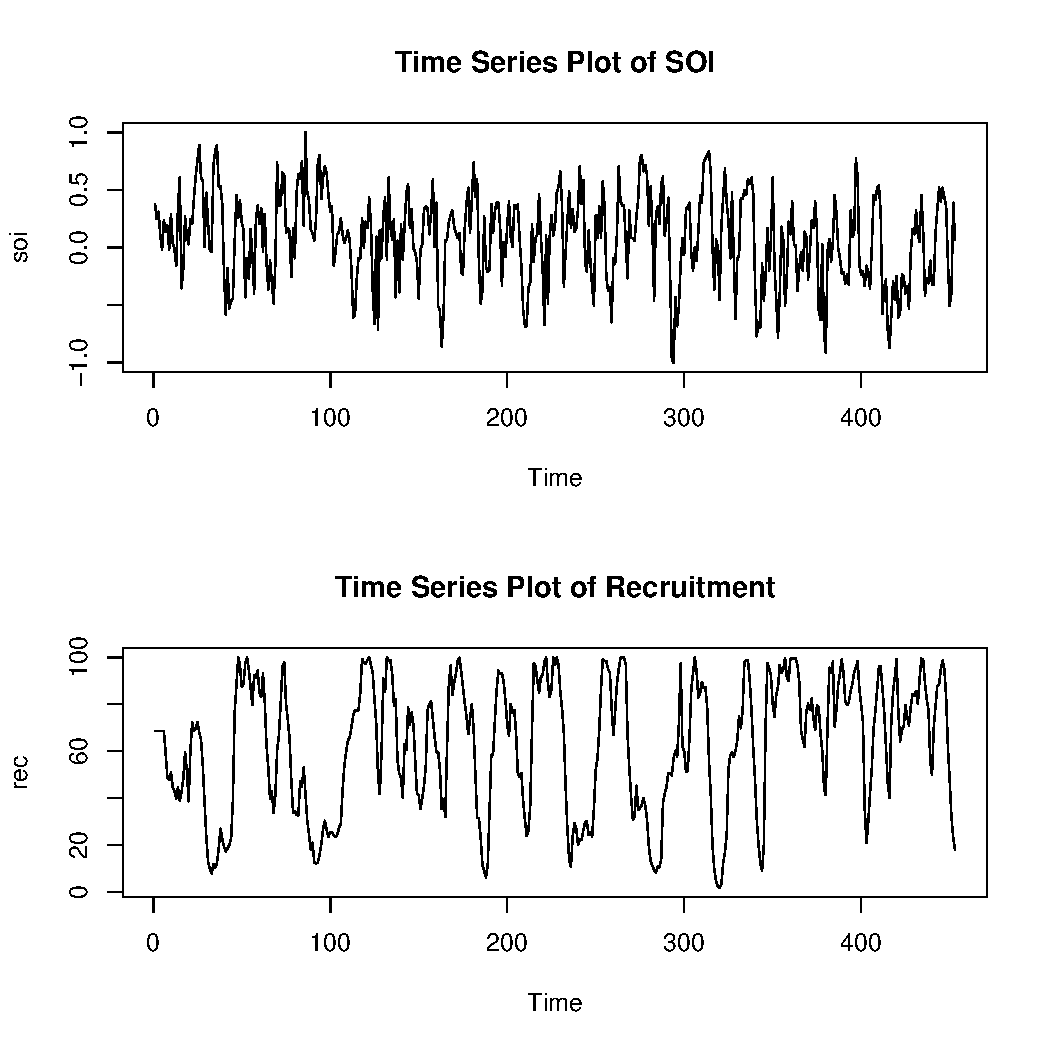
\includegraphics[width=110mm, height=75mm]{ts.pdf}

\end{frame}

\begin{frame}
\frametitle{Worked Example}

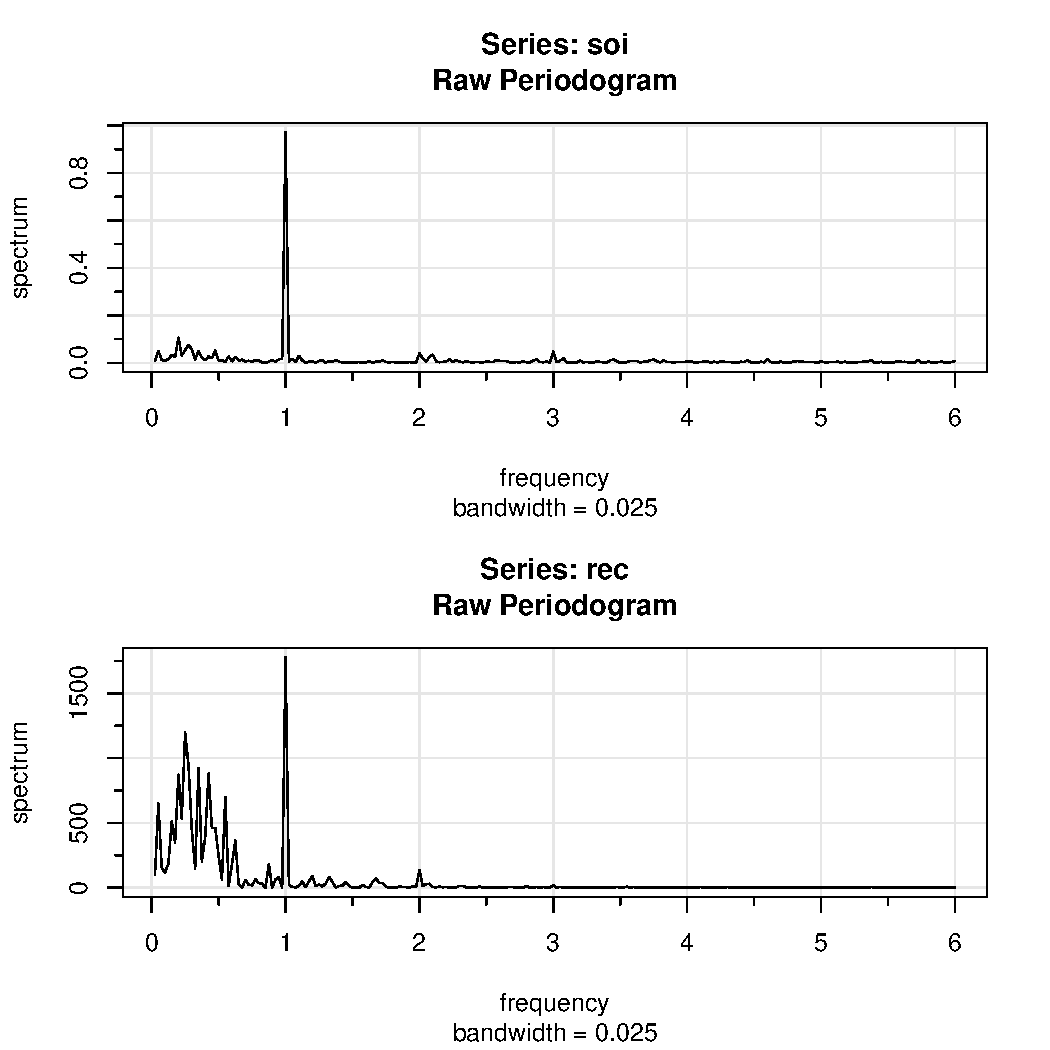
\includegraphics[width=110mm, height=75mm]{periodogram.pdf}

\end{frame}

\begin{frame}
\frametitle{Worked Example}

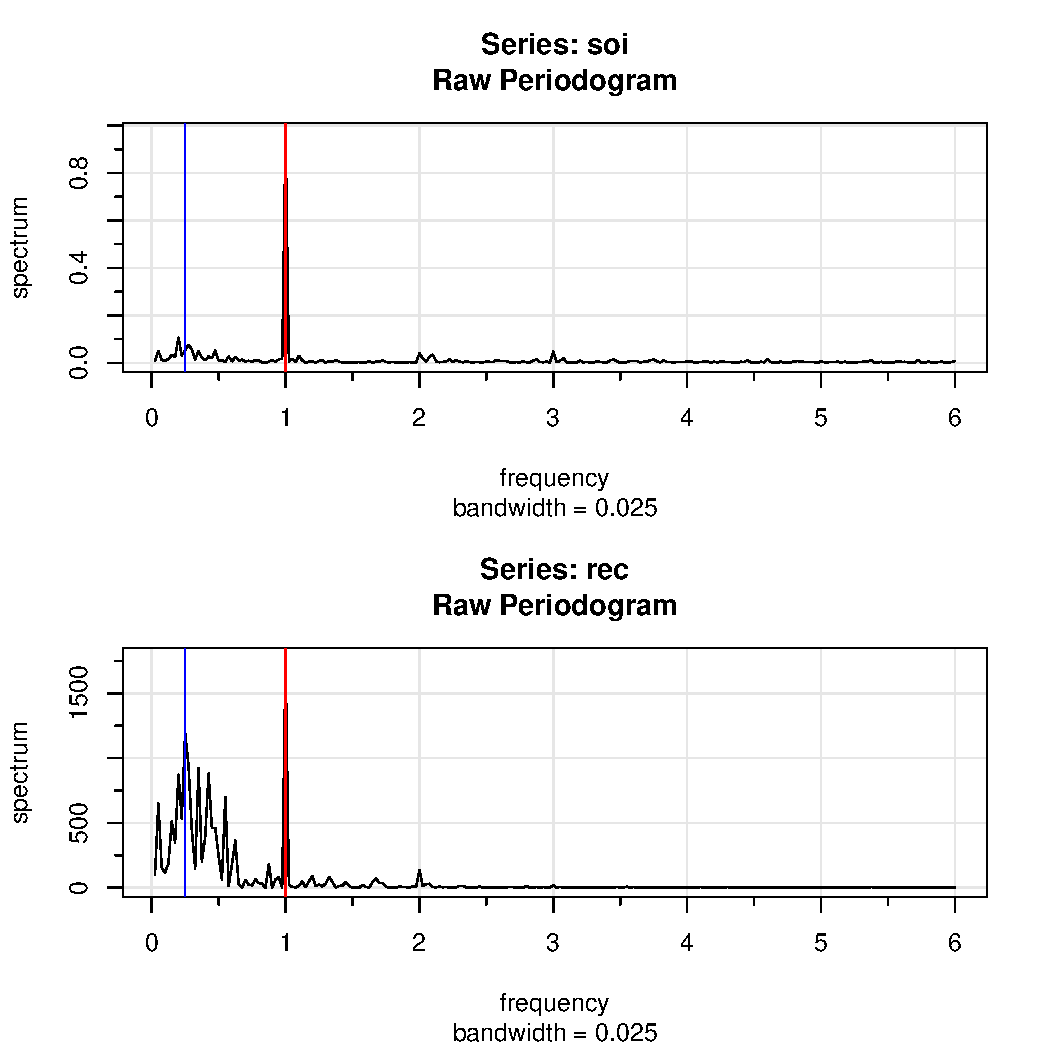
\includegraphics[width=110mm, height=75mm]{periodogram2.pdf}

\end{frame}

\begin{frame} [fragile]
\frametitle{Worked Example}

From the periodograms:

\begin{itemize}
\item obvious peak at $\omega = 1/12$ for yearly cycle.
\item some peaks at around $\omega = 1/48$ for El Nino cycle. The wide band of activity suggests that this cycle is \underline{\hspace{30 mm}}.
\end{itemize}

Note: the horizontal axis of the periodogram produced using the \verb=mvspec()= function from the \verb=astsa= package is in multiples of $\frac{1}{12}$. In Unit 6, the \verb=spec.pgram()= function was used instead and the horizontal axis is the value of the frequency.

\end{frame}

\begin{frame}
\frametitle{Worked Example}

From the SOI data, the value of the periodogram at $\omega = \frac{1}{12}$ is $I(\frac{1}{12}) = 0.9722$. Since $\chi_2^2(0.025) = 0.0506$ and $\chi_2^2(0.975) = 7.3778$, an approximate $95\%$ confidence interval for the spectrum $f(\frac{1}{12})$ is

$$
\left(\frac{2(0.9722)}{7.3778}, \frac{2(0.9722)}{0.0506}\right) = (0.2636, 38.4011).
$$

At $\omega = \frac{1}{48}$, $I(\frac{1}{48}) = 0.0537$, therefore an approximate $95\%$ confidence interval for the spectrum $f(\frac{1}{48})$ is

$$
\left(\frac{2(0.0537)}{7.3778}, \frac{2(0.0537)}{0.0506}\right) = (0.0146, 2.1222).
$$
\end{frame}

\begin{frame}
\frametitle{Worked Example}

\textbf{Question:} Use R to compute $I(\frac{1}{12})$ and $I(\frac{1}{48})$ for the recruit data, as well as derive their corresponding approximate $95\%$ confidence intervals.

\vspace{50mm}

\end{frame}

\end{document} 